\subsection{Minority allocation, softening, and tied maxima}
Table~\ref{tab:primary} compares all four target representations at the same retained count. Figure~\ref{fig:contrasts} shows risk--coverage curves and selected/fixed-epoch contrasts.
\begin{table}[t]
\caption{Selected-checkpoint risk at 80\% common coverage (2,620 of 3,275 images). Risk is mean $\pm$ sample SD across three seeds; components are means in percentage points}\label{tab:primary}
\centering\begin{tabular}{lrrrr}\toprule
Targets & Risk (\%) & Unsupported & Ambiguity & Excess\\\midrule
Hard & $26.30 \pm 1.04$ & 6.65 & 16.14 & 3.51\\
Tie-hard & $25.82 \pm 0.58$ & 6.67 & 16.03 & 3.13\\
Uniform & $24.06 \pm 0.10$ & 6.41 & 15.41 & 2.24\\
Soft & $23.68 \pm 0.07$ & 6.55 & 15.01 & 2.13\\
\bottomrule\end{tabular}
\smallskip\par\footnotesize The three components sum to risk, up to rounding. Accepted identities can differ between models; this is accounting, not causal attribution. Uniform preserves the dominant fraction but spreads remaining supported mass uniformly.
\end{table}

The primary Soft-minus-Uniform difference is -0.38 pp (conditional 95\% interval [-0.64, -0.07]). Paired differences for seeds 17, 42, and 89 are -0.35, -0.43, -0.35 pp. Full soft targets yielded lower selective disagreement than the ambiguity-preserving uniform-minority control under this matched protocol. The retained original Soft-minus-Hard contrast is -2.61 pp (conditional 95\% interval [-2.98, -2.19]). Tie-hard minus Hard is -0.47 pp (conditional 95\% interval [-0.80, -0.12]); Soft minus Tie-hard is -2.14 pp (conditional 95\% interval [-2.49, -1.76]). These latter intervals are descriptive sensitivities, not additional primary hypothesis tests.

\begin{figure}[t]
\centering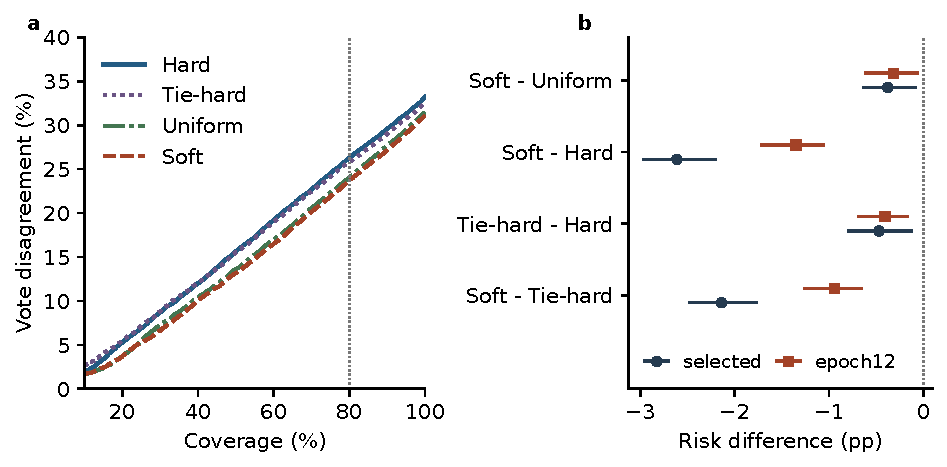
\includegraphics[width=\linewidth]{reviewer_followup/figures/Fig2.pdf}
\caption{(a) Mean selected-checkpoint risk--coverage curves across three seeds; the displayed range begins at 10\%, and every prefix is released. (b) Mean paired contrasts and conditional 95\% pixel-cluster intervals, for selected and epoch-12 weights. Negative differences favor the first-named target. Intervals do not measure seed-population or external-domain uncertainty}\label{fig:contrasts}
\end{figure}
\subsection{Selection sensitivity and label references}
\begin{table}[t]
\caption{Fixed-budget sensitivity and reference-specific metrics. Risk is at 80\% coverage; F1 is at full primary coverage using selected checkpoints. Values are means across three seeds}\label{tab:sensitivity}
\centering\begin{tabular}{lrrrr}\toprule
Targets & Selected & Epoch 12 & Original F1 & Majority F1\\\midrule
Hard & 26.30 & 24.98 & 0.5658 & 0.8965\\
Tie-hard & 25.82 & 24.58 & 0.5599 & 0.9032\\
Uniform & 24.06 & 23.95 & 0.5683 & 0.9205\\
Soft & 23.68 & 23.63 & 0.5722 & 0.9270\\
\bottomrule\end{tabular}
\smallskip\par\footnotesize Risk is a percentage. Both F1 columns are weighted F1, but original labels cover 3,275 images whereas strict crowd-majority labels cover 2,484. Original and crowd-majority labels disagree on 28.46\% of that subset. These F1 values are not interchangeable FER scores. All per-seed values, macro F1, distances, and selected epochs are released.
\end{table}

At fixed epoch 12, Soft minus Uniform is -0.32 pp (conditional 95\% interval [-0.63, -0.05]), and Soft minus Hard is -1.35 pp (conditional 95\% interval [-1.72, -1.05]). Table~\ref{tab:sensitivity} keeps both evaluation states visible. This test changes the stopping decision, not the budget or training objective. The majority-only F1 column concerns a restricted reference task, not an interchangeable performance improvement over original-label F1.

\subsection{Supported mass and the meaning of confidence}
Figure~\ref{fig:mass} separates unsupported mass from ambiguity and excess on each accepted set. Its second panel changes the selection population explicitly rather than silently dropping unsupported votes.
\begin{figure}[t]
\centering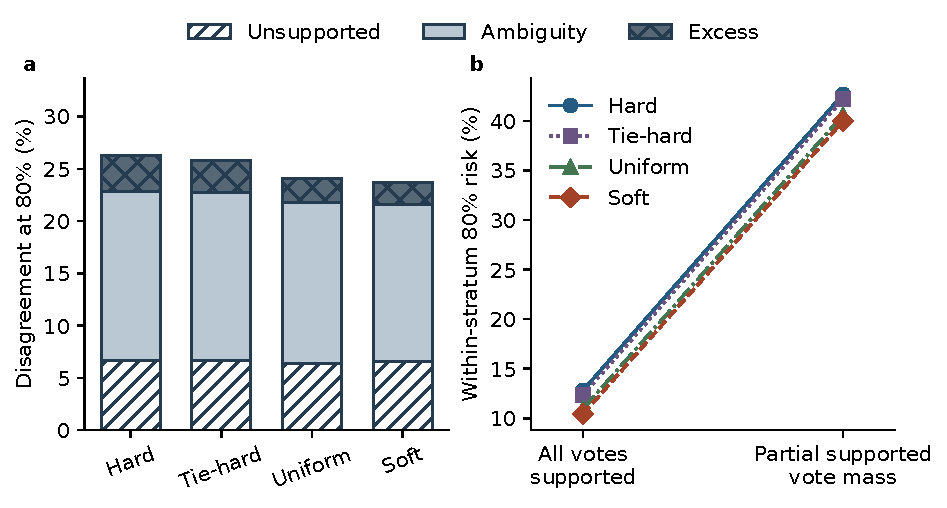
\includegraphics[width=\linewidth]{reviewer_followup/figures/Fig3.pdf}
\caption{(a) Three-way mean risk accounting on global 80\% accepted sets. (b) Independent 80\% selection within full- and partial-supported-mass strata; these populations and vertical scales differ from panel (a). Zero-supported-mass images necessarily have complete-vote risk one and are reported separately in Online Resource 1. Neither panel evaluates an expanded-vocabulary model}\label{fig:mass}
\end{figure}
The primary population contains 1,732 fully supported, 1,527 partially supported, and 16 zero-supported-mass images. Within the fully supported stratum, 80\% risk is 10.42\% for Soft and 10.94\% for Uniform. Within the partially supported stratum, 80\% risk is 40.00\% for Soft and 40.58\% for Uniform. These descriptive comparisons address whether the primary contrast is confined to images with unsupported votes; they do not establish why a model assigned a particular score.

\subsection{Calibration transfer and finite-sample diagnostics}
\begin{table}[t]
\caption{Calibration-fitted policies applied unchanged to primary testing. Entries are mean coverage / risk (\%); coverage includes empty seeds, risk averages nonempty seeds}\label{tab:policies}
\centering\begin{tabular}{llcc}\toprule
Target & Targets & Empirical & Fixed-grid bound\\\midrule
10\% & Hard & 38.35 / 11.45 (3/3) & 0.00 / -- (0/3)\\
10\% & Tie-hard & 39.17 / 11.93 (3/3) & 0.00 / -- (0/3)\\
10\% & Uniform & 45.99 / 12.22 (3/3) & 0.00 / -- (0/3)\\
10\% & Soft & 49.54 / 13.01 (3/3) & 0.00 / -- (0/3)\\
\addlinespace
20\% & Hard & 68.58 / 22.28 (3/3) & 47.03 / 14.55 (3/3)\\
20\% & Tie-hard & 71.04 / 22.80 (3/3) & 48.05 / 14.61 (3/3)\\
20\% & Uniform & 76.20 / 22.80 (3/3) & 57.49 / 16.11 (3/3)\\
20\% & Soft & 76.88 / 22.56 (3/3) & 60.39 / 16.60 (3/3)\\
\addlinespace
30\% & Hard & 98.06 / 32.39 (3/3) & 82.01 / 26.92 (3/3)\\
30\% & Tie-hard & 99.47 / 32.37 (3/3) & 85.41 / 27.54 (3/3)\\
30\% & Uniform & 99.94 / 31.46 (3/3) & 88.41 / 27.11 (3/3)\\
30\% & Soft & 99.91 / 31.07 (3/3) & 89.57 / 27.01 (3/3)\\
\bottomrule\end{tabular}
\smallskip\par\footnotesize Parentheses give nonempty test seeds. An empty policy has undefined risk. Neither a nominal target nor the bound's unverified independence/unchanged-population assumptions establish a deployment guarantee. Different achieved risks are not an equal-risk coverage comparison.
\end{table}

Table~\ref{tab:policies} includes every target and empty-policy outcome. Figure~\ref{fig:transfer} partitions the empirical policy's accepted-population risk change.
\begin{figure}[t]
\centering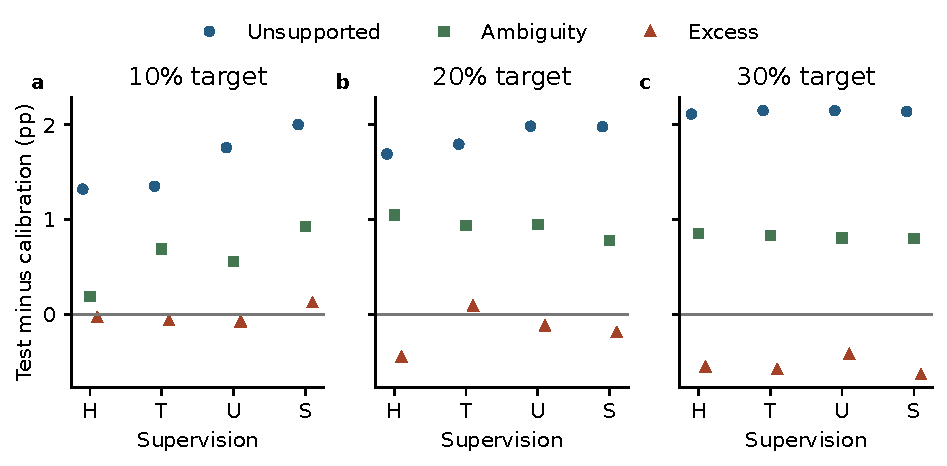
\includegraphics[width=\linewidth]{reviewer_followup/figures/Fig4.pdf}
\caption{Mean test-minus-calibration differences in unsupported mass, supported ambiguity, and excess error for empirical thresholds. Their sum is the risk gap, not a causal attribution. H: Hard; T: Tie-hard; U: Uniform; S: Soft. The three target panels share a vertical scale. Means use paired nonempty calibration/test selections}\label{fig:transfer}
\end{figure}
Across four conditions, 36 of 36 nonempty empirical test operating points exceed their nominal targets. These overlapping outcomes are not independent Bernoulli trials. At the 10\% target, Hard has 38.35\% mean coverage and 11.45\% mean achieved risk. At the 10\% target, Soft has 49.54\% mean coverage and 13.01\% mean achieved risk. Different achieved risks prevent interpreting this as greater coverage at equal risk.

Before confidence selection, the annotation floor is 23.70\% in calibration and 26.67\% in testing: a +2.97 pp difference. Unsupported mass changes from 5.72\% to 7.88\%; the remaining floor difference is supported-category ambiguity. Thus, these populations differ in annotation composition even before a model supplies a ranking.

For Soft at the nominal 20\% target, the accepted test-minus-calibration risk gap is +2.57 pp, comprising +1.98 pp unsupported mass, +0.78 pp supported ambiguity, and -0.19 pp excess. The figure and ledger supply the analogous accounting for every condition and target; this arithmetic does not identify independent causal contributions.

For Hard, the 20\% calibration-half-split holdout-minus-fit risk gap averages +0.05 pp over 300 nonempty seed--split outcomes (descriptive 5th--95th percentiles -2.33 to +2.59 pp). For Tie-hard, the 20\% calibration-half-split holdout-minus-fit risk gap averages +0.18 pp over 300 nonempty seed--split outcomes (descriptive 5th--95th percentiles -2.34 to +2.77 pp). For Uniform, the 20\% calibration-half-split holdout-minus-fit risk gap averages +0.19 pp over 300 nonempty seed--split outcomes (descriptive 5th--95th percentiles -2.02 to +2.62 pp). For Soft, the 20\% calibration-half-split holdout-minus-fit risk gap averages +0.17 pp over 300 nonempty seed--split outcomes (descriptive 5th--95th percentiles -2.00 to +2.43 pp). The complete target-specific resamples are released. These diagnostics reveal within-calibration variability and accepted-population differences, but cannot uniquely separate distribution shift, finite-sample fluctuation, and threshold-search effects.
The fixed-grid comparator yields 24 nonempty test operating points, of which 0 exceed their nominal targets. It abstains completely at the 10\% target for every condition and seed. Its observed conservatism therefore has a concrete coverage cost; these outcomes do not verify its population assumptions.
